% \section{Method}
% \label{sec:method}

% We propose \textbf{Parametric LoRA Updates with Memory Evidence (\method{})}.
% \method{} constructs a global update LoRA to preserve the full context state while emphasizing the latest update, activates query-relevant memory evidence to provide a local parameter view, and adaptively incorporates this local evidence during decoding.

% Figure~\ref{fig:method-overview} provides an overview of the complete \method{} pipeline.
% The upper branch constructs the global update state from the parameter difference between the pre-update and full contexts, while the lower branch activates and parameterizes query-relevant memory evidence.
% Their predictive distributions are combined during adaptive decoding to emphasize currently valid information while retaining unaffected knowledge.

% \begin{figure*}[t]
%     \centering
%     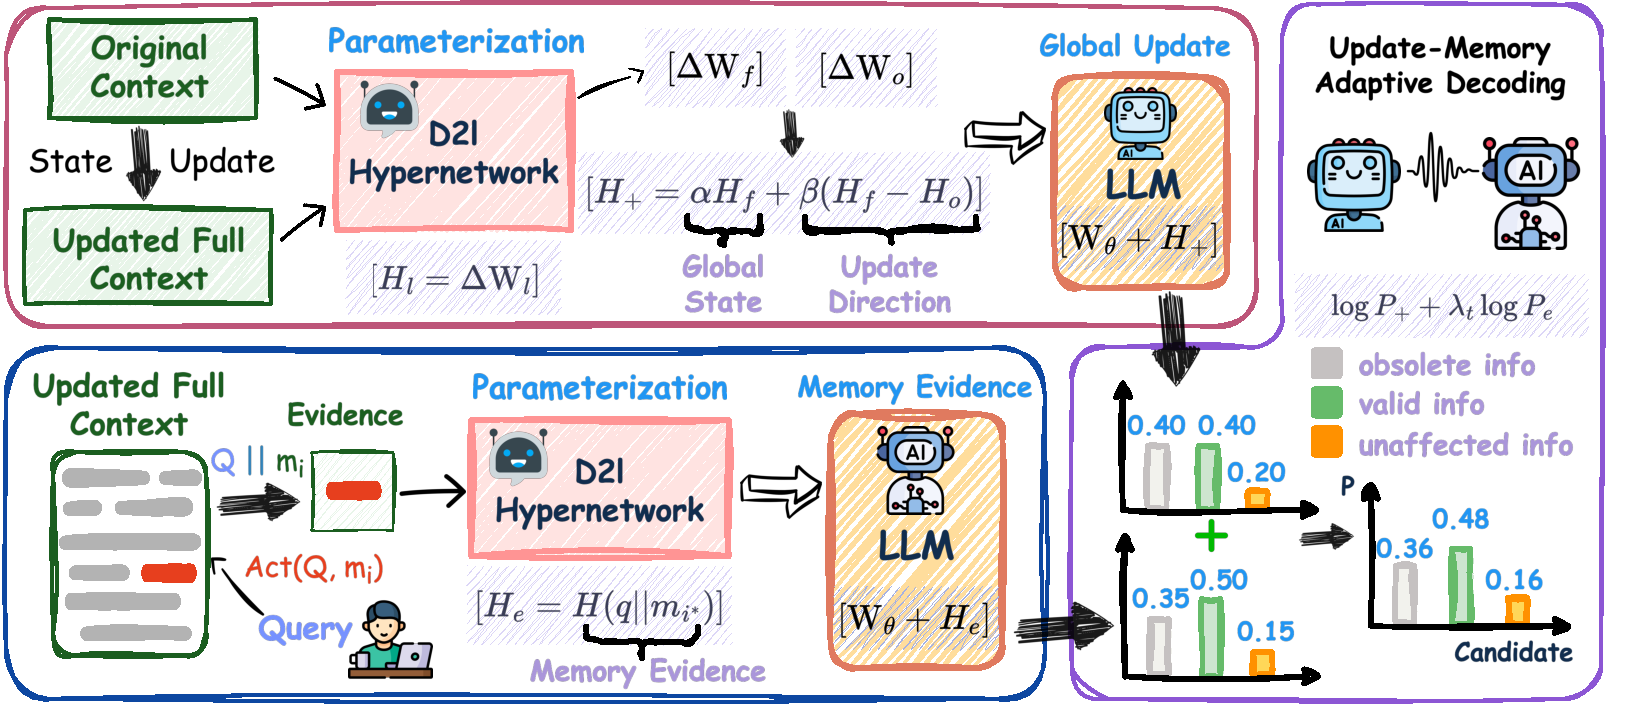
\includegraphics[width=\textwidth]{fig/intro/method.pdf}
%     \caption{Overview of \method{}. The global branch models the parameter change induced by the latest context update, while the memory-evidence branch constructs a query-relevant local parameter view. Adaptive decoding combines their predictions according to the evidence-induced prediction change.}
%     \label{fig:method-overview}
% \end{figure*}


% \subsection{\gur{}}
% \label{sec:global_update_backbone}

% Under continual context updates, a parameterized context may simultaneously encode currently valid, invalidated, and unaffected information.
% To emphasize the latest update while preserving the full context state, we explicitly model the parameter change before and after the update.

% Given the full context history $C_{\mathrm{full}}$ and its pre-update state $C_{\mathrm{old}}$, we parameterize both using the context parameterization hypernetwork $H_\phi$ introduced in Section~\ref{sec:background}, obtaining $\Delta W_{\mathrm{old}}=H_\phi(C_{\mathrm{old}})$ and $\Delta W_{\mathrm{full}}=H_\phi(C_{\mathrm{full}})$.

% Directly using $\Delta W_{\mathrm{full}}$ preserves the complete context history, but may mix information with different validity states.
% In contrast, the difference between the parameter states before and after the update explicitly captures the parameter change induced by the latest update.
% We therefore construct the global update LoRA as
% \begin{equation}
% \Delta W_g
% =
% \alpha \Delta W_{\mathrm{full}}
% +
% \beta
% \left(
% \Delta W_{\mathrm{full}}
% -
% \Delta W_{\mathrm{old}}
% \right),
% \label{eq:global_adapter}
% \end{equation}
% where $\alpha,\beta \geq 0$ are weighting coefficients.
% The first term preserves the overall information encoded by the full context history, while the second amplifies the parameter change induced by the latest update, thereby emphasizing the update direction.

% After applying $\Delta W_g$ to the frozen base model, the global predictive distribution at the $t$-th generation step is
% \begin{equation}
% p_{g,t}(v)
% =
% p_{\theta \oplus \Delta W_g}
% \left(
% v \mid q, y_{<t}
% \right),
% \label{eq:global-distribution}
% \end{equation}
% where $v$ denotes a candidate token, $y_{<t}$ is the previously generated prefix, and $\oplus$ denotes applying the corresponding LoRA adapter to the frozen base model.


% \subsection{\qame{}}
% \label{sec:memory_evidence_activation}

% Although the global update LoRA preserves the full context state, each query typically depends on only a subset of the information contained in the context.
% Relying solely on a unified global parameter state may therefore still introduce interference from information irrelevant to the current query.

% To provide a query-specific local parameter view, we segment $C_{\mathrm{full}}$ into memory units and score each unit according to its lexical relevance to the query.
% The activation score combines query-term coverage with saturated term-frequency matching.
% We select the highest-scoring memory unit as the local memory evidence for the current query, denoted by $m^\star(q)$.
% The query is used only to activate relevant memory evidence and is not passed to the context parameterization hypernetwork.

% We then parameterize the activated memory evidence into an evidence LoRA:
% \begin{equation}
% \Delta W_e(q)
% =
% H_\phi
% \left(
% m^\star(q)
% \right).
% \label{eq:evidence_adapter}
% \end{equation}

% This yields the query-conditioned evidence distribution
% \begin{equation}
% p_{e,t}(v)
% =
% p_{\theta \oplus \Delta W_e(q)}
% \left(
% v \mid q, y_{<t}
% \right).
% \label{eq:evidence-distribution}
% \end{equation}

% Unlike the global LoRA, which encodes the full context history, $\Delta W_e(q)$ captures only the local memory evidence activated for the current query.
% This provides a focused parameter view that emphasizes information directly relevant to the current prediction while reducing interference from unrelated context.


% \subsection{\amd{}}
% \label{sec:adaptive_evidence_decoding}

% The global distribution $p_{g,t}$ provides the complete context state, whereas the evidence distribution $p_{e,t}$ emphasizes local information relevant to the current query.
% However, the contribution of local evidence may vary across generation steps.
% When the local evidence produces predictions similar to the global state, the global prediction is generally sufficient; when it substantially changes the prediction, the local evidence should contribute more strongly.

% We therefore measure the prediction change induced by the local memory evidence using the Jensen--Shannon divergence between the evidence and global distributions:
% \begin{equation}
% d_t
% =
% D_{\mathrm{JS}}
% \left(
% p_{e,t}
% \parallel
% p_{g,t}
% \right).
% \label{eq:js-divergence}
% \end{equation}

% We then convert this divergence into an adaptive evidence weight:
% \begin{equation}
% \lambda_t
% =
% \lambda_{\max}
% \frac{
% d_t
% }{
% d_t+\tau
% },
% \label{eq:adaptive_gate}
% \end{equation}
% where $\lambda_{\max}$ controls the maximum contribution of local evidence and $\tau>0$ controls how rapidly the evidence weight increases with the prediction change.
% A larger divergence results in a larger $\lambda_t$, while similar global and evidence distributions lead to a smaller contribution from the local evidence.

% Finally, we retain the global prediction as the decoding backbone and adaptively augment it with the local evidence prediction:
% \begin{equation}
% S_t(v)
% =
% \log p_{g,t}(v)
% +
% \lambda_t
% \log p_{e,t}(v),
% \label{eq:fusion-score}
% \end{equation}
% where $S_t(v)$ denotes the fused score for token $v$.
% The token with the highest fused score is selected at each generation step.
































% \section{Method}
% \label{sec:method}

% \begin{figure*}[t]
%     \centering
%     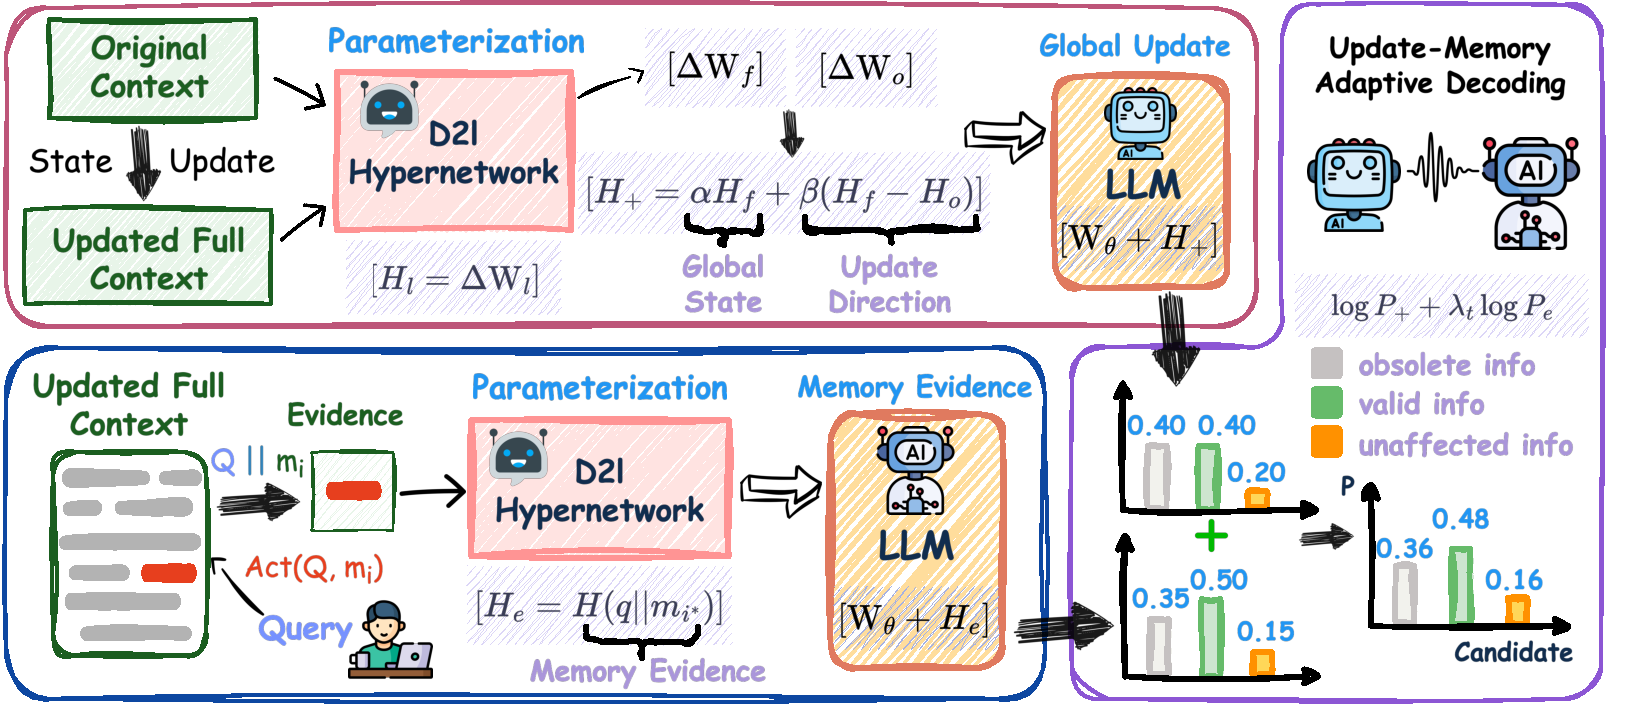
\includegraphics[width=\textwidth]{fig/intro/method.pdf}
%     \captionsetup{justification=raggedright,singlelinecheck=false}
%     \caption{\textbf{The overall framework of our proposed \method{}.}}
%     \label{fig:method-overview}
% \end{figure*}

% We propose \textbf{Parametric LoRA Updates with Memory Evidence (\method{})}.
% \method{} constructs a global update LoRA that preserves the full context state while emphasizing the latest update, activates query-relevant memory evidence as a local parameter view, and adaptively integrates the two during decoding.

% Figure~\ref{fig:method-overview} illustrates the overall pipeline.
% The global branch models the parameter change between the pre-update and full contexts, while the memory-evidence branch parameterizes query-relevant local information.
% Their predictive distributions are adaptively combined to favor currently valid information while preserving unaffected knowledge.



% \subsection{\gur{}}
% \label{sec:global_update_backbone}

% Under continual updates, a parameterized context may simultaneously encode currently valid, invalidated, and unaffected information.
% We therefore model the parameter change induced by the latest update while retaining the full context state.

% Given the full context history $C_{\mathrm{full}}$ and its pre-update state $C_{\mathrm{old}}$, we parameterize both using the context parameterization hypernetwork $H_\phi$ introduced in Section~\ref{sec:background}:
% $\Delta W_{\mathrm{old}}=H_\phi(C_{\mathrm{old}})$ and
% $\Delta W_{\mathrm{full}}=H_\phi(C_{\mathrm{full}})$.

% We construct the global update LoRA as
% \begin{equation}
% \Delta W_g
% =
% \alpha \Delta W_{\mathrm{full}}
% +
% \beta
% \left(
% \Delta W_{\mathrm{full}}
% -
% \Delta W_{\mathrm{old}}
% \right),
% \label{eq:global_adapter}
% \end{equation}
% where $\alpha,\beta \geq 0$ are weighting coefficients.
% The first term preserves the full context state, while the second emphasizes the parameter change induced by the latest update.

% The resulting global predictive distribution at generation step $t$ is
% \begin{equation}
% p_{g,t}(v)
% =
% p_{\theta \oplus \Delta W_g}
% \left(
% v \mid q, y_{<t}
% \right),
% \label{eq:global-distribution}
% \end{equation}
% where $v$ is a candidate token, $y_{<t}$ is the generated prefix, and $\oplus$ denotes applying the LoRA adapter to the frozen base model.


% \subsection{\qame{}}
% \label{sec:memory_evidence_activation}

% A query typically depends on only a subset of the full context, so a unified global parameter state may introduce interference from irrelevant information.
% We therefore construct a query-specific local parameter view.

% We segment $C_{\mathrm{full}}$ into memory units and score them by lexical relevance to the query using query-term coverage and saturated term-frequency matching.
% The highest-scoring unit is selected as the local memory evidence $m^\star(q)$.
% The query is used only for evidence activation and is not passed to the context parameterization hypernetwork.

% The activated evidence is parameterized as
% \begin{equation}
% \Delta W_e(q)
% =
% H_\phi
% \left(
% m^\star(q)
% \right),
% \label{eq:evidence_adapter}
% \end{equation}
% yielding the evidence distribution
% \begin{equation}
% p_{e,t}(v)
% =
% p_{\theta \oplus \Delta W_e(q)}
% \left(
% v \mid q, y_{<t}
% \right).
% \label{eq:evidence-distribution}
% \end{equation}

% Unlike the global LoRA, $\Delta W_e(q)$ captures only query-relevant local evidence, providing a more focused parameter view for the current prediction.

% % Queue the main results table after page 5's top floats have been placed,
% % so that it appears at the top of page 6 before the experiments section.
% % \begingroup

% \definecolor{headerbg}{HTML}{FAF7FF}

% \definecolor{recallarrow}{HTML}{F05A3C}

% \definecolor{llmarrow}{HTML}{3182CE}

% \newcommand{\RecallMetric}{Recall\,\textcolor{recallarrow}{$\uparrow$}}

% \newcommand{\LLMMetric}{LLM\,\textcolor{llmarrow}{$\uparrow$}}

% \newcommand{\PLUMENumber}[1]{{\color{black}\bfseries #1}}

% \newcommand{\SecondNumber}[1]{\uline{#1}}

% \newcommand{\MethodFont}{\fontsize{12pt}{34pt}\selectfont\bfseries}

% \newlength{\ModelHeadingOffset}

% \newlength{\ModelHeadingHeight}

% \newlength{\ModelHeadingAboveSep}

% \newlength{\ModelHeadingBelowSep}

% \setlength{\ModelHeadingOffset}{10.1cm}

% \setlength{\ModelHeadingHeight}{8pt}

% \setlength{\ModelHeadingAboveSep}{0pt}

% \setlength{\ModelHeadingBelowSep}{0pt}

% \newcommand{\ModelHeadingText}[1]{%
%   \makebox[0pt][l]{\hspace*{\ModelHeadingOffset}%
%     {\color{gray}\itshape #1}}%
% }

% \newcommand{\DatasetHeader}[1]{%
%   \begin{tblr}{
%       colspec={Q[c,wd=1.35cm]Q[c,wd=1.05cm]},
%       colsep=3.1pt,
%       rowsep=2pt,
%       rows={font=\bfseries,halign=c,valign=m},
%       hline{2}={wd=0.5pt,solid,leftpos=-0.5,rightpos=-0.5},
%     }
%     \SetCell[c=2]{halign=c,valign=m}#1 & {} \\
%     \RecallMetric & \LLMMetric
%   \end{tblr}%
% }

% \begin{table*}[t]

% \centering

% \small

% \caption{\textbf{Performance comparison of different methods} on five MUSE-Bench datasets across Qwen3 and Gemma-2, evaluated by ROUGE-L Recall and LLM-as-a-Judge.}

% \label{tab:main_results}

% \resizebox{\textwidth}{!}{%

% \begin{tblr}{
%     colspec = {
%         Q[l,wd=4.6cm,valign=m]
%         *{5}{
%             Q[c,wd=1.35cm,valign=m]
%             Q[c,wd=1.05cm,valign=m]
%         }
%     },
%     rowsep = 1pt,
%     % Keep the two rules above each PLUME row distinct after resizing.
%     rulesep = 2pt,
%     colsep = 4pt,
%     row{1} = {bg=headerbg, halign=c, valign=m, font=\bfseries,
%               abovesep=2pt, belowsep=2pt},
%     hline{1} = {wd=2pt, solid},
%     hline{2,11} = {wd=2pt, solid},
%     % The PLUME rows are rows 10 and 19.  Number the two rules explicitly
%     % on those boundaries so they cannot attach to the preceding data row.
%     hline{10,19} = {1}{-}{wd=0.5pt, solid},
%     hline{10,19} = {2}{-}{wd=0.5pt, solid},
%     column{1} = {font=\bfseries},
% }

% \SetCell{halign=c,valign=m}{{\MethodFont Method}}

% & \SetCell[c=2]{halign=c,valign=m}{\DatasetHeader{SQuAD}} & {}

% & \SetCell[c=2]{halign=c,valign=m}{\DatasetHeader{ROPES}} & {}

% & \SetCell[c=2]{halign=c,valign=m}{\DatasetHeader{2Wiki}} & {}

% & \SetCell[c=2]{halign=c,valign=m}{\DatasetHeader{MFQA}} & {}

% & \SetCell[c=2]{halign=c,valign=m}{\DatasetHeader{QASPER}} & {} \\

% \SetRow{ht=\ModelHeadingHeight,
%         abovesep=\ModelHeadingAboveSep,
%         belowsep=\ModelHeadingBelowSep}
% \SetCell[c=11]{halign=l,valign=m}{\ModelHeadingText{Qwen-3}} \\

% \SetHline{1-11}{0.5pt,solid}

% Base Model w/ Context

% & 95.86 & 91.69

% & 97.82 & 95.91

% & 60.11 & 52.35

% & 64.50 & 60.08

% & 61.75 & 53.95

% \\

% Base Model w/o Context

% & 24.61 & 15.19

% & 82.88 & 64.99

% & 31.75 & 24.67

% & 22.48 & 11.33

% & 1.28 & 1.89

% \\

% CD (oracle)

% & 94.93 & 91.75

% & 98.31 & 97.52

% & 68.51 & 65.44

% & 66.24 & 61.17

% & 62.46 & 55.81

% \\

% D2L (oracle)

% & 76.77 & 64.92

% & 85.57 & 80.39

% & 43.13 & 38.33

% & 28.80 & 20.34

% & 22.98 & 15.80

% \\

% CD

% & 40.57 & 27.85

% & 74.69 & 67.00

% & 36.15 & 30.67

% & \SecondNumber{30.78} & \SecondNumber{23.33}

% & 16.78 & 9.57

% \\

% D2L

% & \SecondNumber{54.96} & \SecondNumber{37.27}

% & \SecondNumber{86.99} & \SecondNumber{81.33}

% & \SecondNumber{36.30} & \SecondNumber{30.84}

% & 27.15 & 12.00

% & \SecondNumber{16.88} & \SecondNumber{11.02}

% \\

% AnyEdit (AlphaEdit)

% & 15.77 & 12.44

% & 76.43 & 67.48

% & 16.25 & 15.00

% & 13.23 & 9.25

% & 7.40 & 4.02

% \\

% \SetRow{font=\bfseries\color{black}}

% PLUME

% & \PLUMENumber{80.65} & \PLUMENumber{76.81}

% & \PLUMENumber{94.61} & \PLUMENumber{90.26}

% & \PLUMENumber{47.24} & \PLUMENumber{41.48}

% & \PLUMENumber{37.76} & \PLUMENumber{34.01}

% & \PLUMENumber{28.53} & \PLUMENumber{24.48}

% \\

% \SetRow{ht=\ModelHeadingHeight,
%         abovesep=\ModelHeadingAboveSep,
%         belowsep=\ModelHeadingBelowSep}
% \SetCell[c=11]{halign=l,valign=m}{\ModelHeadingText{Gemma-2}} \\

% \SetHline{1-11}{0.5pt,solid}

% Base Model w/ Context

% & 90.73 & 84.65

% & 84.73 & 80.17

% & 36.39 & 28.21

% & 31.81 & 27.49

% & 52.48 & 44.72

% \\

% Base Model w/o Context

% & 22.07 & 12.54

% & 44.44 & 25.95

% & 14.76 & 6.49

% & 5.02 & 3.36

% & 0.95 & 1.17

% \\

% CD (oracle)

% & 89.92 & 84.77

% & 85.81 & 79.38

% & 42.23 & 34.39

% & 35.11 & 30.84

% & 52.46 & 45.40

% \\

% D2L (oracle)

% & 70.81 & 57.46

% & 58.84 & 50.43

% & 22.11 & 16.15

% & 14.75 & 7.72

% & 19.10 & 12.58

% \\

% CD

% & 32.30 & 20.19

% & 54.63 & 45.21

% & 20.82 & 14.48

% & 9.72 & \SecondNumber{6.76}

% & 12.94 & 5.23

% \\

% D2L

% & \SecondNumber{49.17} & \SecondNumber{31.36}

% & \SecondNumber{57.53} & \SecondNumber{48.69}

% & \SecondNumber{21.09} & \SecondNumber{15.96}

% & \SecondNumber{11.44} & 6.55

% & \SecondNumber{14.22} & \SecondNumber{7.96}

% \\

% AnyEdit (AlphaEdit)

% & 16.24 & 8.93

% & 51.81 & 41.72

% & 10.37 & 8.64

% & 5.23 & 4.06

% & 0.54 & 0.46

% \\

% \SetRow{font=\bfseries\color{black}}

% PLUME

% & \PLUMENumber{74.80} & \PLUMENumber{68.60}

% & \PLUMENumber{62.70} & \PLUMENumber{55.78}

% & \PLUMENumber{29.85} & \PLUMENumber{24.82}

% & \PLUMENumber{23.29} & \PLUMENumber{19.42}

% & \PLUMENumber{24.51} & \PLUMENumber{20.35}

% \\

% \SetHline{1-11}{2pt,solid}

% \end{tblr}%

% }

% \end{table*}

% \endgroup


\begingroup

\definecolor{headerbg}{HTML}{FAF7FF}

\definecolor{recallarrow}{HTML}{F05A3C}

\definecolor{llmarrow}{HTML}{3182CE}

\newcommand{\RecallMetric}{Recall\,\textcolor{recallarrow}{$\uparrow$}}

\newcommand{\LLMMetric}{LLM\,\textcolor{llmarrow}{$\uparrow$}}

\newcommand{\PLUMENumber}[1]{{\color{black}\bfseries #1}}

\newcommand{\SecondNumber}[1]{\uline{#1}}

\newcommand{\MethodFont}{\fontsize{12pt}{34pt}\selectfont\bfseries}

\newlength{\ModelHeadingOffset}

\newlength{\ModelHeadingHeight}

\newlength{\ModelHeadingAboveSep}

\newlength{\ModelHeadingBelowSep}

\setlength{\ModelHeadingOffset}{10.1cm}

\setlength{\ModelHeadingHeight}{8pt}

\setlength{\ModelHeadingAboveSep}{0pt}

\setlength{\ModelHeadingBelowSep}{0pt}

\newcommand{\ModelHeadingText}[1]{%
  \makebox[0pt][l]{\hspace*{\ModelHeadingOffset}%
    {\color{gray}\itshape #1}}%
}

\newcommand{\DatasetHeader}[1]{%
  \begin{tblr}{
      colspec={Q[c,wd=1.35cm]Q[c,wd=1.05cm]},
      colsep=3.1pt,
      rowsep=2pt,
      rows={font=\bfseries,halign=c,valign=m},
      hline{2}={wd=0.5pt,solid,leftpos=-0.5,rightpos=-0.5},
    }
    \SetCell[c=2]{halign=c,valign=m}#1 & {} \\
    \RecallMetric & \LLMMetric
  \end{tblr}%
}

\begin{table*}[t]

\centering

\small

\caption{\textbf{Performance comparison of different methods} on five MUSE-Bench datasets across Qwen3 and Gemma-2, evaluated by ROUGE-L Recall and LLM-as-a-Judge. Oracle methods are excluded when identifying the best and second-best methods.}

\label{tab:main_results}

\resizebox{\textwidth}{!}{%

\begin{tblr}{
    colspec = {
        Q[l,wd=4.6cm,valign=m]
        *{5}{
            Q[c,wd=1.35cm,valign=m]
            Q[c,wd=1.05cm,valign=m]
        }
    },
    rowsep = 1pt,
    % Keep the two rules above each PLUME row distinct after resizing.
    rulesep = 2pt,
    colsep = 4pt,
    row{1} = {bg=headerbg, halign=c, valign=m, font=\bfseries,
              abovesep=2pt, belowsep=2pt},
    hline{1} = {wd=2pt, solid},
    hline{2,11} = {wd=2pt, solid},
    % The PLUME rows are rows 10 and 19.  Number the two rules explicitly
    % on those boundaries so they cannot attach to the preceding data row.
    hline{10,19} = {1}{-}{wd=0.5pt, solid},
    hline{10,19} = {2}{-}{wd=0.5pt, solid},
    column{1} = {font=\bfseries},
}

\SetCell{halign=c,valign=m}{{\MethodFont Method}}

& \SetCell[c=2]{halign=c,valign=m}{\DatasetHeader{SQuAD}} & {}

& \SetCell[c=2]{halign=c,valign=m}{\DatasetHeader{ROPES}} & {}

& \SetCell[c=2]{halign=c,valign=m}{\DatasetHeader{2Wiki}} & {}

& \SetCell[c=2]{halign=c,valign=m}{\DatasetHeader{MFQA}} & {}

& \SetCell[c=2]{halign=c,valign=m}{\DatasetHeader{QASPER}} & {} \\

\SetRow{ht=\ModelHeadingHeight,
        abovesep=\ModelHeadingAboveSep,
        belowsep=\ModelHeadingBelowSep}
\SetCell[c=11]{halign=l,valign=m}{\ModelHeadingText{Qwen-3}} \\

\SetHline{1-11}{0.5pt,solid}

Base w/ Context (oracle)

& 95.86 & 91.69

& 97.82 & 95.91

& 60.11 & 52.35

& 64.50 & 60.08

& 61.75 & 53.95

\\

CD (oracle)

& 94.93 & 91.75

& 98.31 & 97.52

& 68.51 & 65.44

& 66.24 & 61.17

& 62.46 & 55.81

\\

D2L (oracle)

& 76.77 & 64.92

& 85.57 & 80.39

& 43.13 & 38.33

& 28.80 & 20.34

& 22.98 & 15.80

\\

\SetHline{1-11}{0.5pt,solid}

Base w/o Context

& 24.61 & 15.19

& 82.88 & 64.99

& 31.75 & 24.67

& 22.48 & 11.33

& 1.28 & 1.89

\\

AnyEdit

& 15.77 & 12.44

& 76.43 & 67.48

& 16.25 & 15.00

& 13.23 & 9.25

& 7.40 & 4.02

\\

CD

& 40.57 & 27.85

& 74.69 & 67.00

& 36.15 & 30.67

& \SecondNumber{30.78} & \SecondNumber{23.33}

& 16.78 & 9.57

\\

D2L

& \SecondNumber{54.96} & \SecondNumber{37.27}

& \SecondNumber{86.99} & \SecondNumber{81.33}

& \SecondNumber{36.30} & \SecondNumber{30.84}

& 27.15 & 12.00

& \SecondNumber{16.88} & \SecondNumber{11.02}

\\

\SetRow{font=\bfseries\color{black}}

PLUME

& \PLUMENumber{80.65} & \PLUMENumber{76.81}

& \PLUMENumber{94.61} & \PLUMENumber{90.26}

& \PLUMENumber{47.24} & \PLUMENumber{41.48}

& \PLUMENumber{37.76} & \PLUMENumber{34.01}

& \PLUMENumber{28.53} & \PLUMENumber{24.48}

\\

\SetRow{ht=\ModelHeadingHeight,
        abovesep=\ModelHeadingAboveSep,
        belowsep=\ModelHeadingBelowSep}
\SetCell[c=11]{halign=l,valign=m}{\ModelHeadingText{Gemma-2}} \\

\SetHline{1-11}{0.5pt,solid}

Base w/ Context (oracle)

& 90.73 & 84.65

& 84.73 & 80.17

& 36.39 & 28.21

& 31.81 & 27.49

& 52.48 & 44.72

\\

CD (oracle)

& 89.92 & 84.77

& 85.81 & 79.38

& 42.23 & 34.39

& 35.11 & 30.84

& 52.46 & 45.40

\\

D2L (oracle)

& 70.81 & 57.46

& 58.84 & 50.43

& 22.11 & 16.15

& 14.75 & 7.72

& 19.10 & 12.58

\\

\SetHline{1-11}{0.5pt,solid}

Base w/o Context

& 22.07 & 12.54

& 44.44 & 25.95

& 14.76 & 6.49

& 5.02 & 3.36

& 0.95 & 1.17

\\

AnyEdit

& 16.24 & 8.93

& 51.81 & 41.72

& 10.37 & 8.64

& 5.23 & 4.06

& 0.54 & 0.46

\\

CD

& 32.30 & 20.19

& 54.63 & 45.21

& 20.82 & 14.48

& 9.72 & \SecondNumber{6.76}

& 12.94 & 5.23

\\

D2L

& \SecondNumber{49.17} & \SecondNumber{31.36}

& \SecondNumber{57.53} & \SecondNumber{48.69}

& \SecondNumber{21.09} & \SecondNumber{15.96}

& \SecondNumber{11.44} & 6.55

& \SecondNumber{14.22} & \SecondNumber{7.96}

\\

\SetRow{font=\bfseries\color{black}}

PLUME

& \PLUMENumber{74.80} & \PLUMENumber{68.60}

& \PLUMENumber{62.70} & \PLUMENumber{55.78}

& \PLUMENumber{29.85} & \PLUMENumber{24.82}

& \PLUMENumber{23.29} & \PLUMENumber{19.42}

& \PLUMENumber{24.51} & \PLUMENumber{20.35}

\\

\SetHline{1-11}{2pt,solid}

\end{tblr}%

}

\end{table*}

\endgroup



% \subsection{\amd{}}
% \label{sec:adaptive_evidence_decoding}

% The global distribution $p_{g,t}$ preserves the full context state, whereas $p_{e,t}$ emphasizes query-relevant local evidence.
% Because the usefulness of local evidence may vary across generation steps, we adapt its contribution according to the prediction change it induces.

% We measure this change using the Jensen--Shannon divergence:
% \begin{equation}
% d_t=D_{\mathrm{JS}}\left(p_{e,t}\parallelp_{g,t}\right).
% \label{eq:js-divergence}
% \end{equation}

% The adaptive evidence weight is then
% \begin{equation}
% \lambda_t = \lambda_{\max} \frac{d_t}{d_t+\tau},
% \label{eq:adaptive_gate}
% \end{equation}
% where $\lambda_{\max}$ controls the maximum evidence contribution and $\tau>0$ controls its sensitivity to prediction changes.

% Finally, we retain the global prediction as the decoding backbone and augment it with the local evidence:
% \begin{equation}
% S_t(v) = \log p_{g,t}(v) + \lambda_t \log p_{e,t}(v),
% \label{eq:fusion-score}
% \end{equation}
% where $S_t(v)$ is the fused score for token $v$.
% The token with the highest fused score is selected at each generation step.


\section{Method}
\label{sec:method}

\begin{figure*}[t]
    \centering
    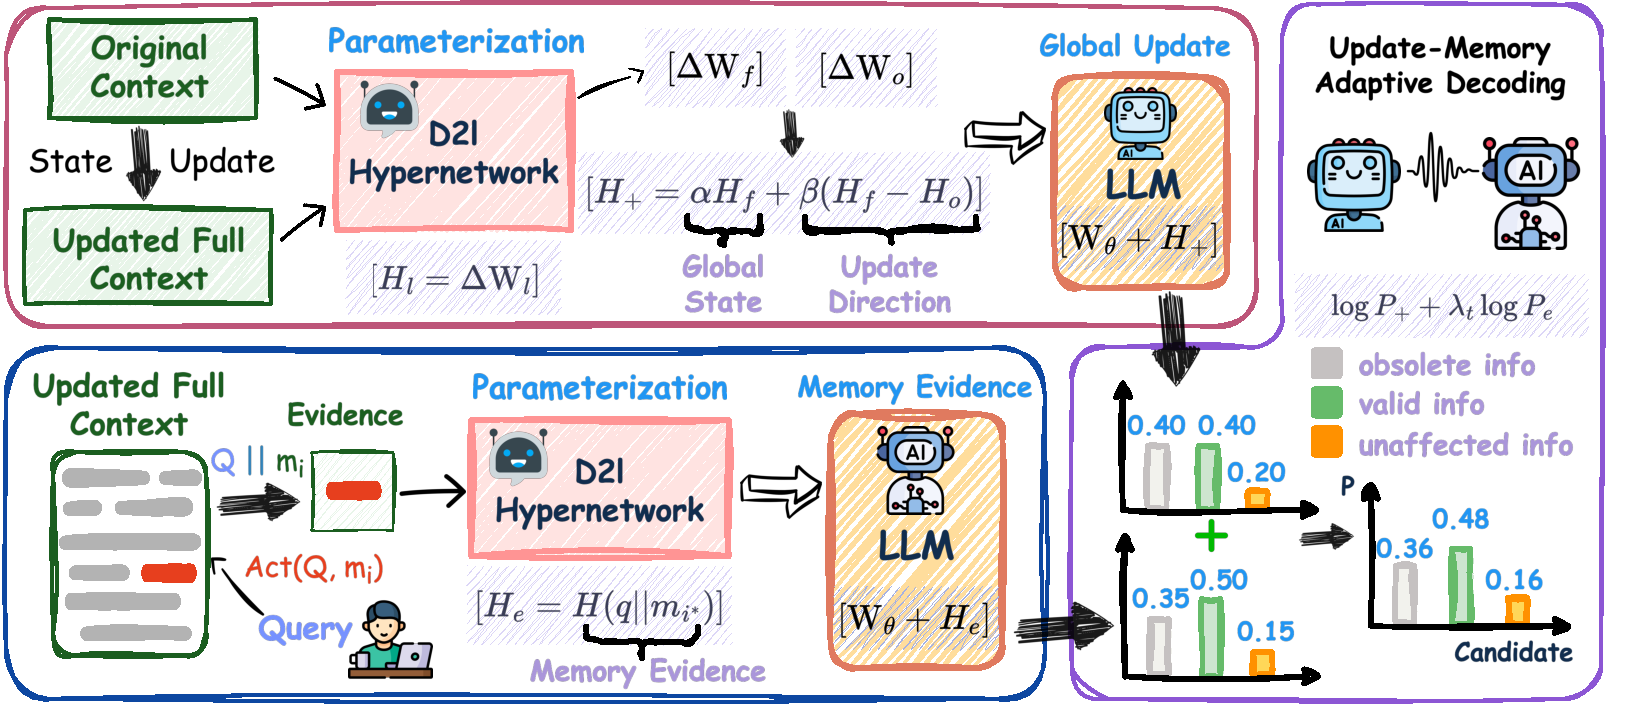
\includegraphics[
        width=\textwidth,
        trim=0 0 15 0,
        clip
    ]{fig/intro/method.pdf}
    \captionsetup{justification=raggedright,singlelinecheck=false}
    \caption{\textbf{The overall framework of our proposed \method{}.} \method{} constructs a global update representation from the full context state, activates memory evidence according to the query to provide a local parameter view, and adaptively integrates the global and local predictions during decoding.
    }
    \label{fig:method-overview}
\end{figure*}

We proposed \textbf{Parametric LoRA Updates with Memory Evidence (\method{})}, which combines a global update representation, query-activated memory evidence, and adaptive decoding for context parameterization under continual updates. Figure~\ref{fig:method-overview} illustrates the overall framework.

\subsection{Global Update Representation}
\label{sec:global_update_backbone}
Under continual updates, a parameterized context may simultaneously encode currently valid, invalid, and unaffected information.
We therefore explicitly model the parameter change induced by the latest update while retaining the full context state. 
Given the full context history $C_{\mathrm{full}}$ and its pre-update state $C_{\mathrm{old}}$, we parameterize them using the context parameterization hypernetwork $H_\phi$ introduced in Section~\ref{sec:background}, obtaining $\Delta W_{\mathrm{old}}=H_\phi(C_{\mathrm{old}})$ and $\Delta W_{\mathrm{full}}=H_\phi(C_{\mathrm{full}})$. 
We then construct the global update representation as
\begin{equation}
\Delta W_g = \alpha \Delta W_{\mathrm{full}} +
\beta\left(\Delta W_{\mathrm{full}}-\Delta W_{\mathrm{old}}\right),
\label{eq:global_adapter}
\end{equation}
where $\alpha,\beta\geq0$ are weighting coefficients.
The first term retains the full context state, while the second emphasizes the parameter change induced by the latest update. 
The resulting global update representation therefore preserves the complete parameterized state while strengthening the latest update. 
At generation step $t$, its predictive distribution is
\begin{equation}
p_{g,t}(v) = p_{\theta\oplus\Delta W_g} \left(v\mid q,y_{<t}\right),
\label{eq:global-distribution}
\end{equation}
where $v$ denotes a candidate token, $y_{<t}$ is the generated prefix, and $\oplus$ denotes applying the corresponding parameter update to the frozen base model.


\subsection{\qame{}}
\label{sec:memory_evidence_activation}

A query typically depends on only a small portion of the full context, while a unified global parameter state may introduce interference from irrelevant information. We therefore construct a query-specific local parameter view by segmenting $C_{\mathrm{full}}$ into memory units at a fine semantic granularity and scoring their lexical relevance to the query based on query-term coverage and saturated term-frequency matching. The highest-scoring unit is activated as the local memory evidence $m^\star(q)$. The query is used only for evidence activation and is not provided to the context parameterization hypernetwork. The memory evidence is parameterized as
\begin{equation}
\Delta W_e(q)=H_\phi\left(m^\star(q)\right),
\label{eq:evidence_adapter}
\end{equation}
with the corresponding predictive distribution
\begin{equation}
p_{e,t}(v) = p_{\theta\oplus\Delta W_e(q)} \left(v\mid q,y_{<t}\right).
\label{eq:evidence-distribution}
\end{equation}
Unlike the global update representation, $\Delta W_e(q)$ parameterizes only the query-activated memory evidence, forming a local parameterized state for the current query. This local state provides complementary information to the full context representation and helps reduce interference from information unrelated to the current prediction.

% \begingroup

% \definecolor{headerbg}{HTML}{FAF7FF}

% \definecolor{recallarrow}{HTML}{F05A3C}

% \definecolor{llmarrow}{HTML}{3182CE}

% \newcommand{\RecallMetric}{Recall\,\textcolor{recallarrow}{$\uparrow$}}

% \newcommand{\LLMMetric}{LLM\,\textcolor{llmarrow}{$\uparrow$}}

% \newcommand{\PLUMENumber}[1]{{\color{black}\bfseries #1}}

% \newcommand{\SecondNumber}[1]{\uline{#1}}

% \newcommand{\MethodFont}{\fontsize{12pt}{34pt}\selectfont\bfseries}

% \newlength{\ModelHeadingOffset}

% \newlength{\ModelHeadingHeight}

% \newlength{\ModelHeadingAboveSep}

% \newlength{\ModelHeadingBelowSep}

% \setlength{\ModelHeadingOffset}{10.1cm}

% \setlength{\ModelHeadingHeight}{8pt}

% \setlength{\ModelHeadingAboveSep}{0pt}

% \setlength{\ModelHeadingBelowSep}{0pt}

% \newcommand{\ModelHeadingText}[1]{%
%   \makebox[0pt][l]{\hspace*{\ModelHeadingOffset}%
%     {\color{gray}\itshape #1}}%
% }

% \newcommand{\DatasetHeader}[1]{%
%   \begin{tblr}{
%       colspec={Q[c,wd=1.35cm]Q[c,wd=1.05cm]},
%       colsep=3.1pt,
%       rowsep=2pt,
%       rows={font=\bfseries,halign=c,valign=m},
%       hline{2}={wd=0.5pt,solid,leftpos=-0.5,rightpos=-0.5},
%     }
%     \SetCell[c=2]{halign=c,valign=m}#1 & {} \\
%     \RecallMetric & \LLMMetric
%   \end{tblr}%
% }

% \begin{table*}[t]

% \centering

% \small

% \caption{\textbf{Performance comparison of different methods} on five MUSE-Bench datasets across Qwen3 and Gemma-2, evaluated by ROUGE-L Recall and LLM-as-a-Judge.}

% \label{tab:main_results}

% \resizebox{\textwidth}{!}{%

% \begin{tblr}{
%     colspec = {
%         Q[l,wd=4.6cm,valign=m]
%         *{5}{
%             Q[c,wd=1.35cm,valign=m]
%             Q[c,wd=1.05cm,valign=m]
%         }
%     },
%     rowsep = 1pt,
%     % Keep the two rules above each PLUME row distinct after resizing.
%     rulesep = 2pt,
%     colsep = 4pt,
%     row{1} = {bg=headerbg, halign=c, valign=m, font=\bfseries,
%               abovesep=2pt, belowsep=2pt},
%     hline{1} = {wd=2pt, solid},
%     hline{2,11} = {wd=2pt, solid},
%     % The PLUME rows are rows 10 and 19.  Number the two rules explicitly
%     % on those boundaries so they cannot attach to the preceding data row.
%     hline{10,19} = {1}{-}{wd=0.5pt, solid},
%     hline{10,19} = {2}{-}{wd=0.5pt, solid},
%     column{1} = {font=\bfseries},
% }

% \SetCell{halign=c,valign=m}{{\MethodFont Method}}

% & \SetCell[c=2]{halign=c,valign=m}{\DatasetHeader{SQuAD}} & {}

% & \SetCell[c=2]{halign=c,valign=m}{\DatasetHeader{ROPES}} & {}

% & \SetCell[c=2]{halign=c,valign=m}{\DatasetHeader{2Wiki}} & {}

% & \SetCell[c=2]{halign=c,valign=m}{\DatasetHeader{MFQA}} & {}

% & \SetCell[c=2]{halign=c,valign=m}{\DatasetHeader{QASPER}} & {} \\

% \SetRow{ht=\ModelHeadingHeight,
%         abovesep=\ModelHeadingAboveSep,
%         belowsep=\ModelHeadingBelowSep}
% \SetCell[c=11]{halign=l,valign=m}{\ModelHeadingText{Qwen-3}} \\

% \SetHline{1-11}{0.5pt,solid}

% Base Model w/ Context

% & 95.86 & 91.69

% & 97.82 & 95.91

% & 60.11 & 52.35

% & 64.50 & 60.08

% & 61.75 & 53.95

% \\

% Base Model w/o Context

% & 24.61 & 15.19

% & 82.88 & 64.99

% & 31.75 & 24.67

% & 22.48 & 11.33

% & 1.28 & 1.89

% \\

% CD (oracle)

% & 94.93 & 91.75

% & 98.31 & 97.52

% & 68.51 & 65.44

% & 66.24 & 61.17

% & 62.46 & 55.81

% \\

% D2L (oracle)

% & 76.77 & 64.92

% & 85.57 & 80.39

% & 43.13 & 38.33

% & 28.80 & 20.34

% & 22.98 & 15.80

% \\

% CD

% & 40.57 & 27.85

% & 74.69 & 67.00

% & 36.15 & 30.67

% & \SecondNumber{30.78} & \SecondNumber{23.33}

% & 16.78 & 9.57

% \\

% D2L

% & \SecondNumber{54.96} & \SecondNumber{37.27}

% & \SecondNumber{86.99} & \SecondNumber{81.33}

% & \SecondNumber{36.30} & \SecondNumber{30.84}

% & 27.15 & 12.00

% & \SecondNumber{16.88} & \SecondNumber{11.02}

% \\

% AnyEdit (AlphaEdit)

% & 15.77 & 12.44

% & 76.43 & 67.48

% & 16.25 & 15.00

% & 13.23 & 9.25

% & 7.40 & 4.02

% \\

% \SetRow{font=\bfseries\color{black}}

% PLUME

% & \PLUMENumber{80.65} & \PLUMENumber{76.81}

% & \PLUMENumber{94.61} & \PLUMENumber{90.26}

% & \PLUMENumber{47.24} & \PLUMENumber{41.48}

% & \PLUMENumber{37.76} & \PLUMENumber{34.01}

% & \PLUMENumber{28.53} & \PLUMENumber{24.48}

% \\

% \SetRow{ht=\ModelHeadingHeight,
%         abovesep=\ModelHeadingAboveSep,
%         belowsep=\ModelHeadingBelowSep}
% \SetCell[c=11]{halign=l,valign=m}{\ModelHeadingText{Gemma-2}} \\

% \SetHline{1-11}{0.5pt,solid}

% Base Model w/ Context

% & 90.73 & 84.65

% & 84.73 & 80.17

% & 36.39 & 28.21

% & 31.81 & 27.49

% & 52.48 & 44.72

% \\

% Base Model w/o Context

% & 22.07 & 12.54

% & 44.44 & 25.95

% & 14.76 & 6.49

% & 5.02 & 3.36

% & 0.95 & 1.17

% \\

% CD (oracle)

% & 89.92 & 84.77

% & 85.81 & 79.38

% & 42.23 & 34.39

% & 35.11 & 30.84

% & 52.46 & 45.40

% \\

% D2L (oracle)

% & 70.81 & 57.46

% & 58.84 & 50.43

% & 22.11 & 16.15

% & 14.75 & 7.72

% & 19.10 & 12.58

% \\

% CD

% & 32.30 & 20.19

% & 54.63 & 45.21

% & 20.82 & 14.48

% & 9.72 & \SecondNumber{6.76}

% & 12.94 & 5.23

% \\

% D2L

% & \SecondNumber{49.17} & \SecondNumber{31.36}

% & \SecondNumber{57.53} & \SecondNumber{48.69}

% & \SecondNumber{21.09} & \SecondNumber{15.96}

% & \SecondNumber{11.44} & 6.55

% & \SecondNumber{14.22} & \SecondNumber{7.96}

% \\

% AnyEdit (AlphaEdit)

% & 16.24 & 8.93

% & 51.81 & 41.72

% & 10.37 & 8.64

% & 5.23 & 4.06

% & 0.54 & 0.46

% \\

% \SetRow{font=\bfseries\color{black}}

% PLUME

% & \PLUMENumber{74.80} & \PLUMENumber{68.60}

% & \PLUMENumber{62.70} & \PLUMENumber{55.78}

% & \PLUMENumber{29.85} & \PLUMENumber{24.82}

% & \PLUMENumber{23.29} & \PLUMENumber{19.42}

% & \PLUMENumber{24.51} & \PLUMENumber{20.35}

% \\

% \SetHline{1-11}{2pt,solid}

% \end{tblr}%

% }

% \end{table*}

% \endgroup


\begingroup

\definecolor{headerbg}{HTML}{FAF7FF}

\definecolor{recallarrow}{HTML}{F05A3C}

\definecolor{llmarrow}{HTML}{3182CE}

\newcommand{\RecallMetric}{Recall\,\textcolor{recallarrow}{$\uparrow$}}

\newcommand{\LLMMetric}{LLM\,\textcolor{llmarrow}{$\uparrow$}}

\newcommand{\PLUMENumber}[1]{{\color{black}\bfseries #1}}

\newcommand{\SecondNumber}[1]{\uline{#1}}

\newcommand{\MethodFont}{\fontsize{12pt}{34pt}\selectfont\bfseries}

\newlength{\ModelHeadingOffset}

\newlength{\ModelHeadingHeight}

\newlength{\ModelHeadingAboveSep}

\newlength{\ModelHeadingBelowSep}

\setlength{\ModelHeadingOffset}{10.1cm}

\setlength{\ModelHeadingHeight}{8pt}

\setlength{\ModelHeadingAboveSep}{0pt}

\setlength{\ModelHeadingBelowSep}{0pt}

\newcommand{\ModelHeadingText}[1]{%
  \makebox[0pt][l]{\hspace*{\ModelHeadingOffset}%
    {\color{gray}\itshape #1}}%
}

\newcommand{\DatasetHeader}[1]{%
  \begin{tblr}{
      colspec={Q[c,wd=1.35cm]Q[c,wd=1.05cm]},
      colsep=3.1pt,
      rowsep=2pt,
      rows={font=\bfseries,halign=c,valign=m},
      hline{2}={wd=0.5pt,solid,leftpos=-0.5,rightpos=-0.5},
    }
    \SetCell[c=2]{halign=c,valign=m}#1 & {} \\
    \RecallMetric & \LLMMetric
  \end{tblr}%
}

\begin{table*}[t]

\centering

\small

\caption{\textbf{Performance comparison of different methods} on five MUSE-Bench datasets across Qwen3 and Gemma-2, evaluated by ROUGE-L Recall and LLM-as-a-Judge. Oracle methods are excluded when identifying the best and second-best methods.}

\label{tab:main_results}

\resizebox{\textwidth}{!}{%

\begin{tblr}{
    colspec = {
        Q[l,wd=4.6cm,valign=m]
        *{5}{
            Q[c,wd=1.35cm,valign=m]
            Q[c,wd=1.05cm,valign=m]
        }
    },
    rowsep = 1pt,
    % Keep the two rules above each PLUME row distinct after resizing.
    rulesep = 2pt,
    colsep = 4pt,
    row{1} = {bg=headerbg, halign=c, valign=m, font=\bfseries,
              abovesep=2pt, belowsep=2pt},
    hline{1} = {wd=2pt, solid},
    hline{2,11} = {wd=2pt, solid},
    % The PLUME rows are rows 10 and 19.  Number the two rules explicitly
    % on those boundaries so they cannot attach to the preceding data row.
    hline{10,19} = {1}{-}{wd=0.5pt, solid},
    hline{10,19} = {2}{-}{wd=0.5pt, solid},
    column{1} = {font=\bfseries},
}

\SetCell{halign=c,valign=m}{{\MethodFont Method}}

& \SetCell[c=2]{halign=c,valign=m}{\DatasetHeader{SQuAD}} & {}

& \SetCell[c=2]{halign=c,valign=m}{\DatasetHeader{ROPES}} & {}

& \SetCell[c=2]{halign=c,valign=m}{\DatasetHeader{2Wiki}} & {}

& \SetCell[c=2]{halign=c,valign=m}{\DatasetHeader{MFQA}} & {}

& \SetCell[c=2]{halign=c,valign=m}{\DatasetHeader{QASPER}} & {} \\

\SetRow{ht=\ModelHeadingHeight,
        abovesep=\ModelHeadingAboveSep,
        belowsep=\ModelHeadingBelowSep}
\SetCell[c=11]{halign=l,valign=m}{\ModelHeadingText{Qwen-3}} \\

\SetHline{1-11}{0.5pt,solid}

Base w/ Context (oracle)

& 95.86 & 91.69

& 97.82 & 95.91

& 60.11 & 52.35

& 64.50 & 60.08

& 61.75 & 53.95

\\

CD (oracle)

& 94.93 & 91.75

& 98.31 & 97.52

& 68.51 & 65.44

& 66.24 & 61.17

& 62.46 & 55.81

\\

D2L (oracle)

& 76.77 & 64.92

& 85.57 & 80.39

& 43.13 & 38.33

& 28.80 & 20.34

& 22.98 & 15.80

\\

\SetHline{1-11}{0.5pt,solid}

Base w/o Context

& 24.61 & 15.19

& 82.88 & 64.99

& 31.75 & 24.67

& 22.48 & 11.33

& 1.28 & 1.89

\\

AnyEdit

& 15.77 & 12.44

& 76.43 & 67.48

& 16.25 & 15.00

& 13.23 & 9.25

& 7.40 & 4.02

\\

CD

& 40.57 & 27.85

& 74.69 & 67.00

& 36.15 & 30.67

& \SecondNumber{30.78} & \SecondNumber{23.33}

& 16.78 & 9.57

\\

D2L

& \SecondNumber{54.96} & \SecondNumber{37.27}

& \SecondNumber{86.99} & \SecondNumber{81.33}

& \SecondNumber{36.30} & \SecondNumber{30.84}

& 27.15 & 12.00

& \SecondNumber{16.88} & \SecondNumber{11.02}

\\

\SetRow{font=\bfseries\color{black}}

PLUME

& \PLUMENumber{80.65} & \PLUMENumber{76.81}

& \PLUMENumber{94.61} & \PLUMENumber{90.26}

& \PLUMENumber{47.24} & \PLUMENumber{41.48}

& \PLUMENumber{37.76} & \PLUMENumber{34.01}

& \PLUMENumber{28.53} & \PLUMENumber{24.48}

\\

\SetRow{ht=\ModelHeadingHeight,
        abovesep=\ModelHeadingAboveSep,
        belowsep=\ModelHeadingBelowSep}
\SetCell[c=11]{halign=l,valign=m}{\ModelHeadingText{Gemma-2}} \\

\SetHline{1-11}{0.5pt,solid}

Base w/ Context (oracle)

& 90.73 & 84.65

& 84.73 & 80.17

& 36.39 & 28.21

& 31.81 & 27.49

& 52.48 & 44.72

\\

CD (oracle)

& 89.92 & 84.77

& 85.81 & 79.38

& 42.23 & 34.39

& 35.11 & 30.84

& 52.46 & 45.40

\\

D2L (oracle)

& 70.81 & 57.46

& 58.84 & 50.43

& 22.11 & 16.15

& 14.75 & 7.72

& 19.10 & 12.58

\\

\SetHline{1-11}{0.5pt,solid}

Base w/o Context

& 22.07 & 12.54

& 44.44 & 25.95

& 14.76 & 6.49

& 5.02 & 3.36

& 0.95 & 1.17

\\

AnyEdit

& 16.24 & 8.93

& 51.81 & 41.72

& 10.37 & 8.64

& 5.23 & 4.06

& 0.54 & 0.46

\\

CD

& 32.30 & 20.19

& 54.63 & 45.21

& 20.82 & 14.48

& 9.72 & \SecondNumber{6.76}

& 12.94 & 5.23

\\

D2L

& \SecondNumber{49.17} & \SecondNumber{31.36}

& \SecondNumber{57.53} & \SecondNumber{48.69}

& \SecondNumber{21.09} & \SecondNumber{15.96}

& \SecondNumber{11.44} & 6.55

& \SecondNumber{14.22} & \SecondNumber{7.96}

\\

\SetRow{font=\bfseries\color{black}}

PLUME

& \PLUMENumber{74.80} & \PLUMENumber{68.60}

& \PLUMENumber{62.70} & \PLUMENumber{55.78}

& \PLUMENumber{29.85} & \PLUMENumber{24.82}

& \PLUMENumber{23.29} & \PLUMENumber{19.42}

& \PLUMENumber{24.51} & \PLUMENumber{20.35}

\\

\SetHline{1-11}{2pt,solid}

\end{tblr}%

}

\end{table*}

\endgroup



% \subsection{\amd{}}
% \label{sec:adaptive_evidence_decoding}

% The global distribution $p_{g,t}$ captures the full context state, whereas $p_{e,t}$ provides query-specific local evidence. Because the contribution of local evidence may vary across generation steps, we adaptively weight it according to the prediction difference between the two distributions. Specifically, we compute their Jensen--Shannon divergence as
% \begin{equation}
% d_t
% =
% D_{\mathrm{JS}}\left(p_{e,t}\parallel p_{g,t}\right),
% \label{eq:js-divergence}
% \end{equation}
% and define the adaptive evidence weight as
% \begin{equation}
% \lambda_t
% =
% \lambda_{\max}\frac{d_t}{d_t+\tau},
% \label{eq:adaptive_gate}
% \end{equation}
% where $\lambda_{\max}$ controls the maximum evidence contribution and $\tau>0$ determines the sensitivity to prediction differences.

% We retain the global prediction as the decoding backbone and incorporate the local evidence through
% \begin{equation}
% S_t(v)
% =
% \log p_{g,t}(v)
% +
% \lambda_t\log p_{e,t}(v),
% \label{eq:fusion-score}
% \end{equation}
% where $S_t(v)$ denotes the fused score for token $v$. The token with the highest fused score is selected at each generation step.


\subsection{\amd{}}
\label{sec:adaptive_evidence_decoding}

The global distribution $p_{g,t}$ is induced by the global update representation and reflects the full parameterized context state, whereas $p_{e,t}$ is induced by the query-activated memory evidence and provides a complementary local parameterized state. Since the contribution of the activated evidence may vary across generation steps, we adaptively determine its influence according to the distributional difference between the two predictions. Specifically, we measure this difference using the JS divergence:
\begin{equation}
d_t = D_{\mathrm{JS}}\left(p_{e,t}\parallel p_{g,t}\right),
\label{eq:js-divergence}
\end{equation}
and define the adaptive evidence weight as
\begin{equation}
\lambda_t = \lambda_{\max}\frac{d_t}{d_t+\tau},
\label{eq:adaptive_gate}
\end{equation}
where $\lambda_{\max}$ controls the maximum contribution of the activated evidence and $\tau>0$ controls the sensitivity of the adaptive weighting to distributional differences across generation steps.

We retain the global prediction as the decoding backbone and incorporate the activated memory evidence through
\begin{equation}
S_t(v) = \log p_{g,t}(v) + \lambda_t\log p_{e,t}(v),
\label{eq:fusion-score}
\end{equation}
where $S_t(v)$ denotes the fused score for token $v$. In this way, the global update representation preserves the full context state, while the activated memory evidence provides additional local information when it induces a meaningful prediction change. The token with the highest fused score is selected at each generation step.
